\documentclass[aspectratio=43]{beamer}

\usepackage[T1]{fontenc}
\usepackage[utf8x]{inputenc}
\usepackage[ngerman]{babel}
\usepackage{amsfonts,amsmath,amssymb,amsthm}
\usepackage{csquotes}

\usepackage{hyperref}

\usetheme[komms=false]{fbmathematik}

%%%%%%%%%%%%%%%%%%%%%%%%%%%%%%%%%%%%%%%%%%%%%%%%%%%%%%%%%%%
% Schriftfarben:
% tuklblau, tuklrot, warmgrau, kaltgrau;
% abgeschwächte Töne für die obigen Farben und schwarz:
% z.B. tuklblau7 für 70% tuklblau, warmgrau2 für 20%
% warmgrau oder schwarz6 für 60% schwarz,
% jeweils in den Schritten 10%, 20%, 40%, 60%, 70%, 80%;
% violette Schriftfarbe (Felix-Klein) hat den Namen fkz1
% hellviolette FKZ-Variante hat den Namen fkz2;
% KOMMS: kommsblau, kommsgruen, kommsgrau, kommsblaugrau
%%%%%%%%%%%%%%%%%%%%%%%%%%%%%%%%%%%%%%%%%%%%%%%%%%%%%%%%%%%



\title{Immer der Sonn' entgegen}
\subtitle{3. Zwischenbericht}
\author{Dominik Bendle \and Melissa Hasel \and Thomas Hofmann}
\date{\today}
\institute{TU Kaiserslautern}

\begin{document}

\begin{frame}[plain]

    % Leerzeilen vor und nach Titel sind offenbar nötig
    \Titel{logo}

\end{frame}

\begin{frame}
    \frametitle{Höhendaten reloaded}
    \begin{itemize}
        \item Modell mit Einbezug von Höhendaten wies in letzter Version Fehler auf
        \item[] $\rightarrow$ Fehler bei Einheitenumrechnung, Eingabe verfälscht
        \item Weiteres Problem: eher geringe Datendichte (ca.90\,m zwischen
            Koordinatenpunkten)
        \item vorherige Lösung: nimm nächstgelegenen Höhenwert
        \item jetzt: lineare Interpolation
        \item wegen bessere Funktionalität: auch ins OSM-Modell eingebaut
    \end{itemize}
\end{frame}

\begin{frame}
    \frametitle{Beispiele}
    \begin{figure}[t]
        \centering
        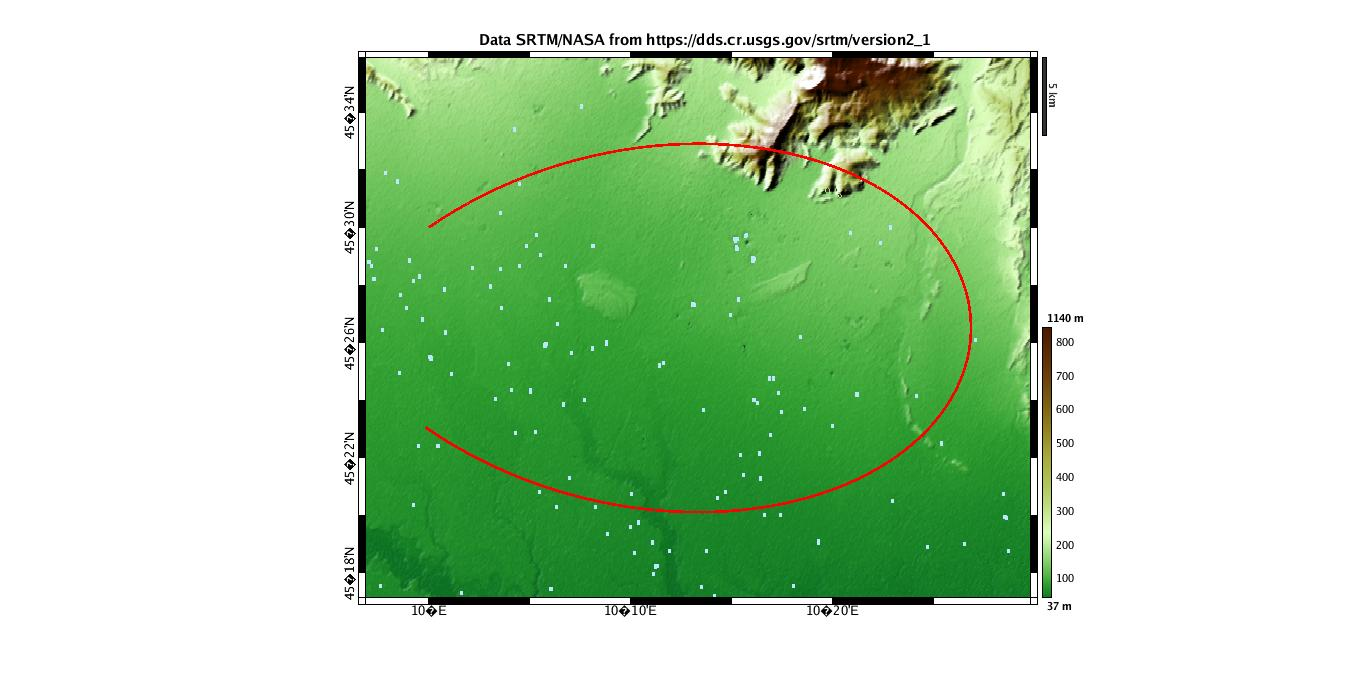
\includegraphics[width=0.95\textwidth]{bilder/nostreetnoele.jpg}
        \caption{Ohne Berücksichtigung der Höhe}
    \end{figure}
\end{frame}

\begin{frame}
    \frametitle{Beispiele}
    \begin{figure}[t]
        \centering
        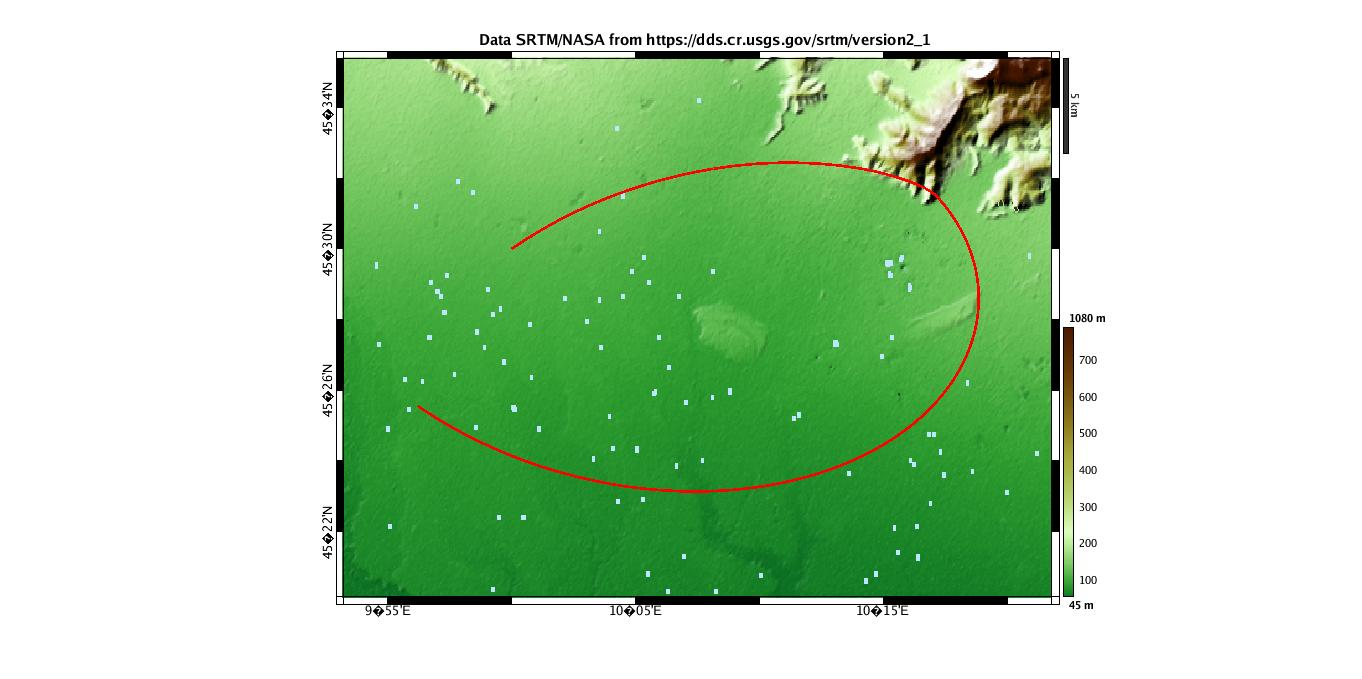
\includegraphics[width=0.95\textwidth]{bilder/nostreetele.jpg}
        \caption{Mit Berücksichtigung der Höhe}
    \end{figure}
\end{frame}

\begin{frame}
    \frametitle{Änderungen am Laufmodell}
    Vorher
    \begin{itemize}
        \item An Kreuzung nimm gehe nur weiter wenn Straßen nicht von Sonne weg führen
        \item[] $\rightarrow$ bleiben in bestimmten Straßen für lange Zeit stecken
    \end{itemize}
    Nun
    \begin{itemize}
        \item wähle nun an einer Kreuzung immer einen Weg, auch wenn er von der Sonne
            wegführt
        \item mache nun niemals kehrt, d.h. gehe niemals in Richtung des zuletzt besuchten
            Knotens
    \end{itemize}
    Dies verhindert das Steckenbleiben in bestimmten Wegen, können aber dennoch in
    Rundwegen lange im Kreis laufen
\end{frame}

\begin{frame}
    \frametitle{Präsentation der Daten im OSM-Modell}
\end{frame}

\begin{frame}
    \frametitle{Beispiele}
    \begin{figure}[t]
        \centering
        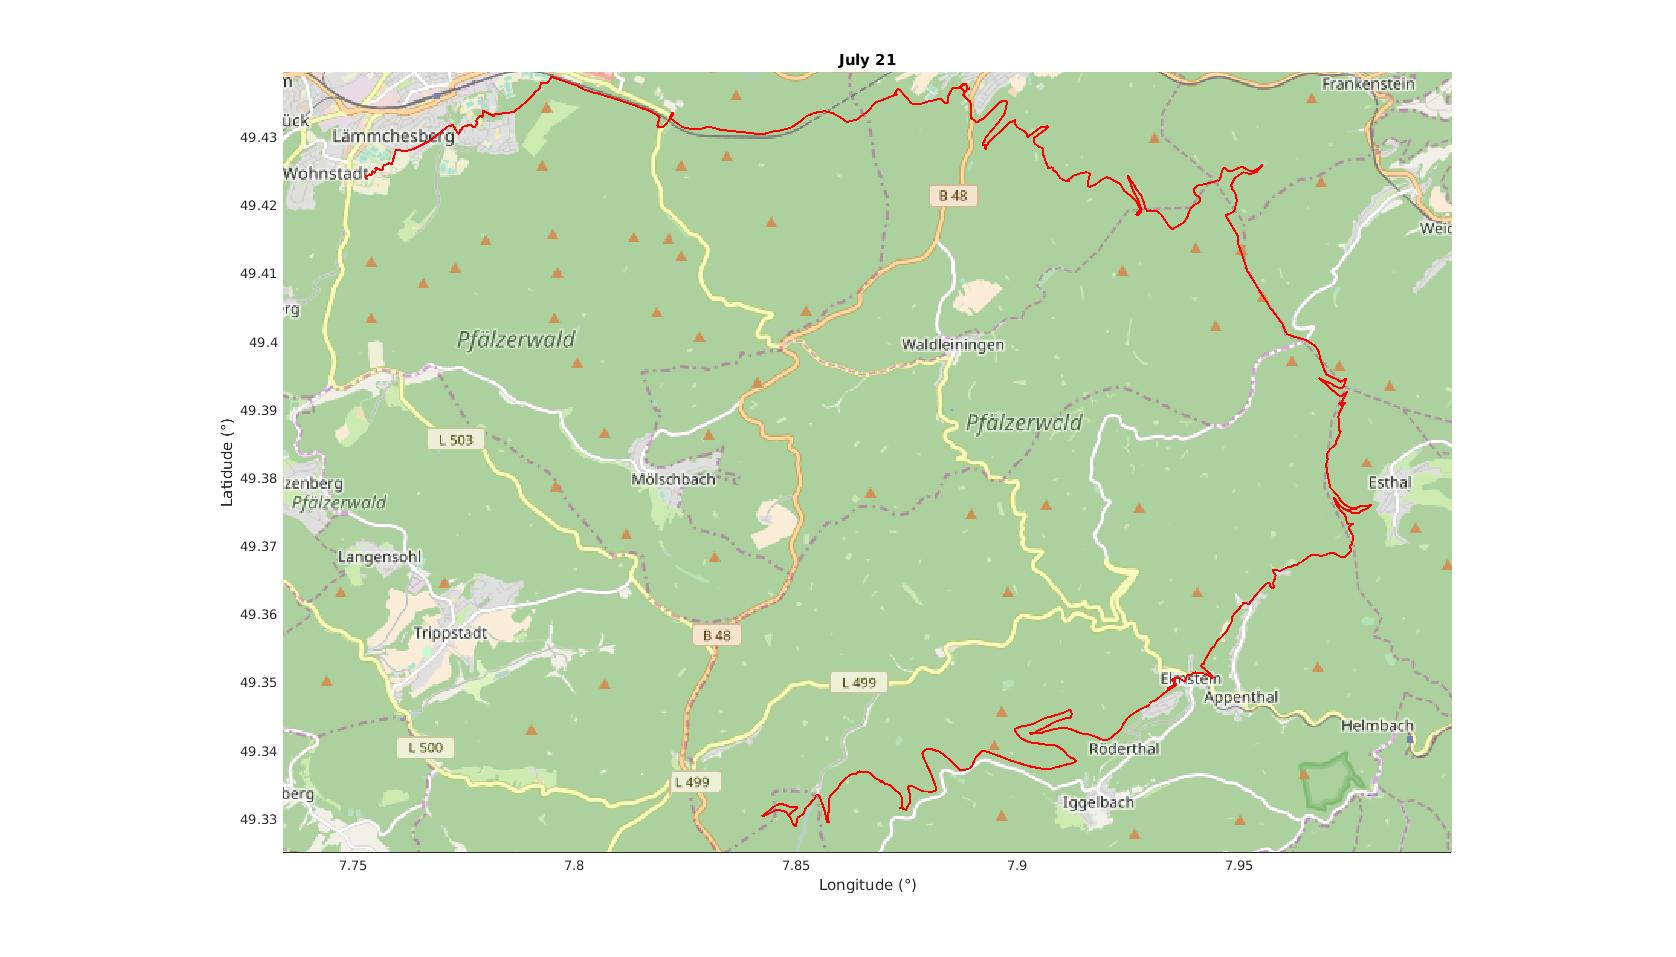
\includegraphics[width=0.95\textwidth]{bilder/noele.jpg}
        \caption{Ohne Berücksichtigung der Höhe}
    \end{figure}
\end{frame}

\begin{frame}
    \frametitle{Beispiele}
    \begin{figure}[t]
        \centering
        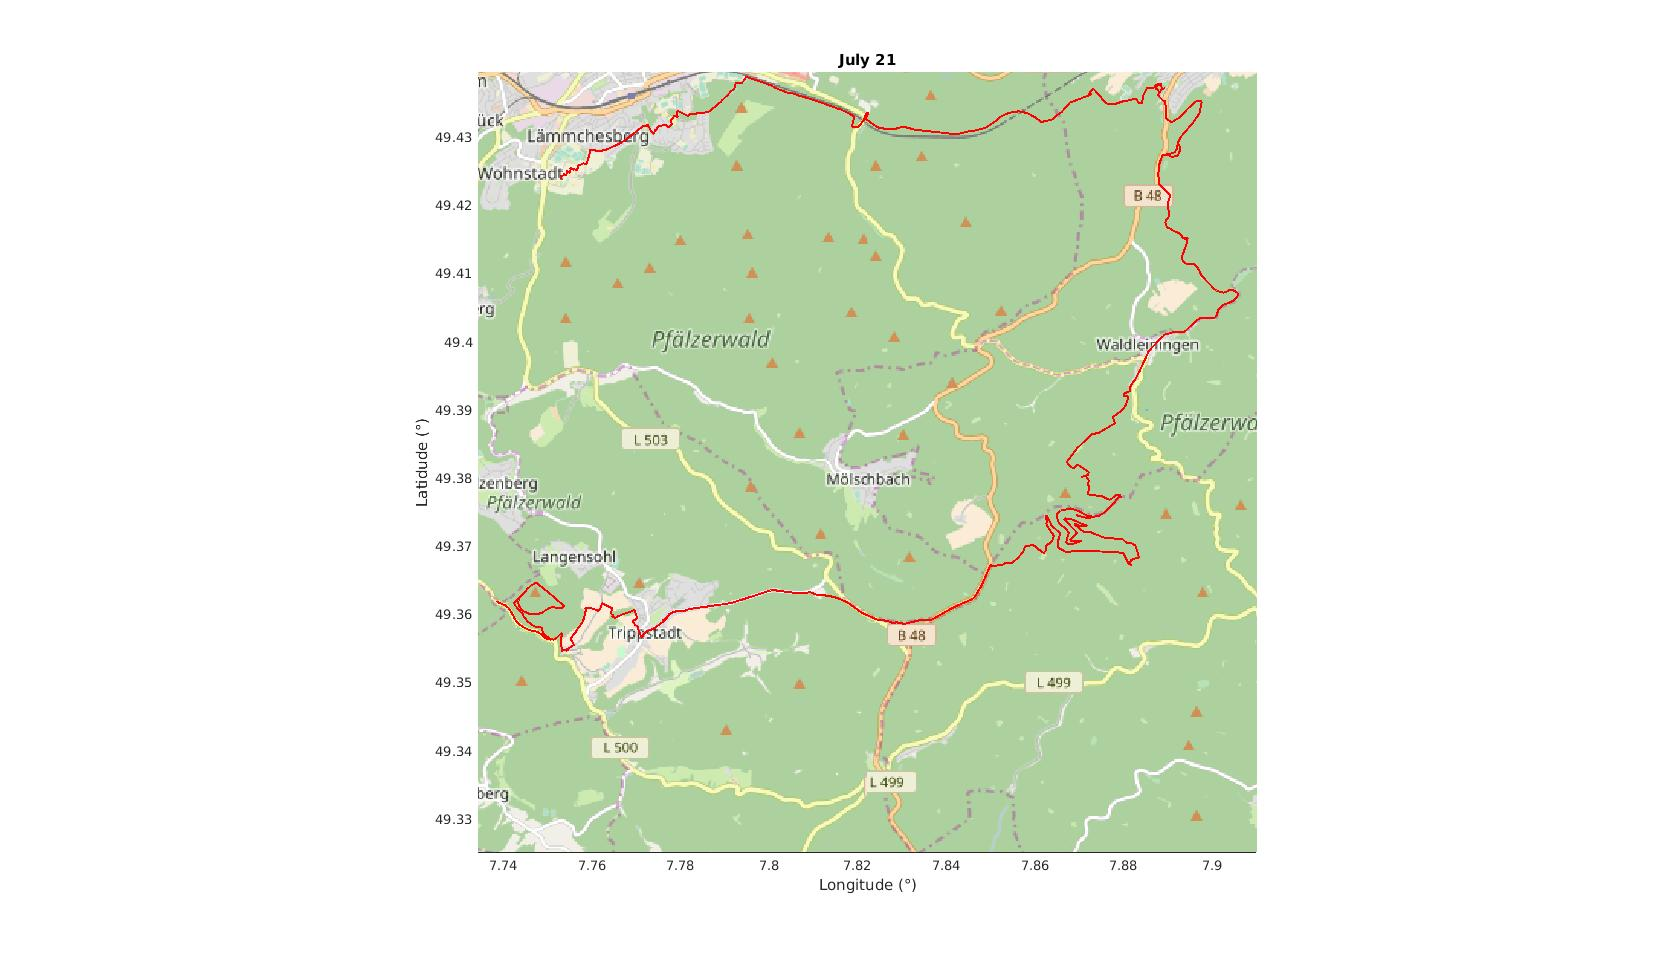
\includegraphics[width=0.95\textwidth]{bilder/ele.jpg}
        \caption{Mit Berücksichtigung der Höhe}
    \end{figure}
\end{frame}

\end{document}
